\chapter{简介和起因}
机器学习和设计从数据中自动提取有价值信息的算法息息相关。
这里的重点在于"自动",
i.e., 当处理有意义的事物时, 机器学习关注可以用于多个数据集(dataset)的通用方法论(general-purpose methodologies).
机器学习有三个核心概念: 数据, 模型, 学习(data, a model, and learning).

\marginpar{数据}
因为机器学习本身就是数据驱动的, 数据是机器学习的核心。
机器学习的目的就是设计通用方法来从数据中提取有价值的模式(patterns), 理想情况下不需要太多领域特定知识。
例如, 给定一个大型文档语料库(e.g., 许多图书馆的书), 机器学习方法能够自动查找相关主题, 这些主题是跨文档共享的(Hoffman et al., 2010).
\marginpar{模型}
为了实现这个目的, 我们设计通常和生成数据过程相关的模型, 和我们给定的数据集类似。
例如, 在回归中, 模型描述一个函数, 该函数映射输入到一个实值输出。
转述Mitchell(1997): 如果在考虑数据后模型在给定任务上的性能有所提高,则称该模型从数据中学习。
目的是找到能够很好的概括未知数据(即, 泛化能力强)的好模型, 这我们以后或许会关心。
\marginpar{学习}
学习可以理解为一种通过优化模型参数自动寻找数据中模式和结构的方式。

机器学习已经有过许多成功案例, 设计和训练复杂而灵活的机器学习系统的软件一应俱全。
我们相信这本机器学习数学基础对于理解基础原则是十分重要的, 更复杂的机器学习系统都构建在这些基础原则上。
理解这些原则能够促进创建新的机器学习解决方案, 理解和调试已经存在的方法, 和学习方法学固有的假设和局限

\section{凭直觉理解单词}
在机器学习中我们经常遇到的一个挑战就是那些概念和单词都十分棘手,
并且一个机器学习系统的特定部分会被抽象为不同的数学概念。
例如, 单词"算法(algorithm)"在机器学习语境中至少有两个不同的应用场景。
第一个场景中, 我们用短语"机器学习算法"代表一个根据输入数据做出预测的系统。
我们称这些算法为预测器(predictors).\marginpar{预测器}
第二个场景中, 我们用相同的短语"机器学习算法"代表一个适应预测器内部参数的系统, 这样它在处理未知输入数据时能表现良好。
我们称这种适应为"训练"一个系统。\marginpar{训练}

这本书不会解决歧义问题, 但我们希望预先强调这些: 取决于上下文, 相同的表述可能意味着不同的事物。
虽然如此, 我们将尝试给出一个清晰的上下文以减少歧义。

这本书的第一部分介绍了关于机器学习三大概念:数据,模型, 学习需要知道的数学概念和数学基础。
我们在这里简要的列出大纲, 当我们讨论必须的数学概念时, 我们会再看到他们。

因为并非所有数据都是以数字表示的, 将数据视作数字格式常常有用。
本书中, 我们假设数据已经被恰当的转换为数字表示并且适合被计算机程序读取。
所以, 我们可以将数据视为向量 \marginpar{将数据视作向量}.
作为另一个说明词是多么微妙的例子, (至少)有三种不同的方式来思考向量:
向量是一个数字数组(计算机科学视角),
向量是一个有大小和方向的箭头(物理视角),
向量是一个服从加法(addition)和乘法(scaling)的对象(数学视角)。

一个模型\marginpar{模型}经常被用来描述生成数据的过程, 类似于手头的数据集。
因此, 好的模型会被视作简化版本的真实(未知)数据生成过程, 从中获取数据建模和提取隐藏模式相关的方面。
一个好的模型没有在真实世界实验就可以很好的预测真实世界会发生什么。

现在我们到了问题的关键--机器学习中的学习\marginpar{学习}.
假设我们给定了一个数据集和合适的模型。
训练这个模型意味着使用可获取的数据依据效用函数(utility functioin)优化模型的一些参数,
效用函数估计出模型预测训练数据有多好。
多数训练方法可以看作是一种爬山登顶的方法。
在这个比喻中, 峰顶对应着一些你希望的性能指标的最大化。
然而, 在实践中, 我们对模型处理未知数据表现良好的模型很感兴趣。
在处理我们已知的数据(训练数据)中表现良好, 可能仅仅意味着我们找到了一个很好的方法来记忆数据。
但是, 这不能很好的泛化到未知数据, 并且不能实际应用, 我们经常需要机器学习系统处于他从未遇到过的环境中。

让我们总结一下我们在本书中介绍的机器学习中的重要概念:

\begin{itemize}
	\item 我们将数据视作向量
	\item 我们选择恰当的模型, 无论从概率视角或优化视角
	\item 我们从可获取的数据中使用数学优化方法学习, 目的是在接受非训练数据时也能表现良好
\end{itemize}

\section{阅读本书的两种方式}

我们有两种策略来理解机器学习中的数学:

\begin{itemize}
	\item \textbf{自底向上:}
	从基础开始到高级逐渐构建概念。 这在学习技术领域是最好的方法, 例如数学。
	这种策略的优点是读者可以在任意时刻回顾先前学习的概念。
	不幸的是, 对于学习者, 许多基础概念对他们来说并不十分有趣, 而缺少动机意味着大量的基本定义会很快遗忘。
	\item \textbf{自顶向下:}
	从实践中钻研需要更多基础需求。
	这类目标驱动方式有着自己的优点:在任何时刻,读者都知道为什么他们需要研究某一概念, 并且明确获取所需知识的途径。
	这种策略的缺点是知识可能构建在不稳定的基础之上, 读者需要记忆一系列他们没有办法理解单词。
\end{itemize}

我们决定以模块化的方式写这本书, 这样分开(数学的)基础概念, 读者就可以以上面两种方式阅读本书了。
这本书分为两部分, 第一部分奠定数学基础, 第二部分应用从第一部分学到的概念解决一些基础的机器学习问题,
这些问题形成机器学习的四大支柱(参见 图1.1):
回归(regression), 降维(demensionality), 密度估计(density estimation), 和分类(classification).
第一部分的章节多数都构建在前一章之上, 但是跳过某一章并在需要时跳回阅读是可能的。
第二部分的章节都是松耦合的(loosely coupled)所以可以以任何顺序阅读。
在两部分间有许多向前向后的提示以将数学概念和机器学习算法联系起来。

\begin{figure}
	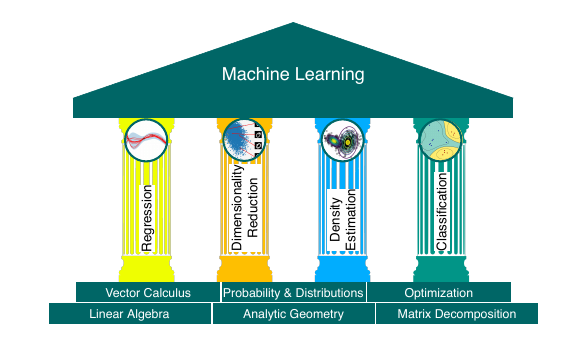
\includegraphics[width=\textwidth]{./chapter01/pillar.png}
	\caption{基石和机器学习四大支柱}
\end{figure}

当然有更多其他方式阅读这本书。
多数读者学习时采用自底向上和自顶向下结合的方式,
有时在尝试复杂概念时先学习基础的数学技巧,
也选择基于机器学习应用的主题进行学习。

\begin{center} 第一部分关于数学 \end{center}
我们在本书中要学习机器学习的四大支柱需要有坚实的数学基础, 这些分布在第一部分中。

我们将数值数据(numerical data)表示为向量, 将这样的数据的表格表示为矩阵。
研究向量和矩阵的就是线性代数, 我们将在第二章介绍。\marginpar{线性代数}
作为向量集合的矩阵也在这里讲述。

给定两个向量来表示真实世界的两个对象, 我们想要对它们的相似性发表看法。
这个想法是:相似的向量通过我们的机器学习算法(预测器)应当能被预测到有相似的输出。
为了形式化这个两向量间相似性的想法, 我们需要介绍一种运算,将两个向量作为输入, 返回一个数值来表示他们的相似性的。
相似的构造和距离是解析几何的重心, 这将在第三章讨论。\marginpar{解析几何}

在第四章, 我们会介绍一些关于矩阵和矩阵分解的基础概念。
一些矩阵运算在机器学习中极其有用, 也允许对数据和更有效的学习进行直觉上的解释。\marginpar{矩阵分解}

我们经常认为数据是对潜在的真实信号的有噪音的观察。
我们希望通过应用机器学习我们可以从噪音中识别信号。
这要求我们有一门语言来量化"噪音"到底是什么。
我们也经常喜欢用允许我们表达某种程度不确定性的预测器来量化我们在特定测试数据点上关于预测值的置信度。
量化不确定性是概率论的领域, 这会在第六章覆盖。\marginpar{概率论}

为了训练机器学习模型, 我们通常寻找使得性能测量最大化的参数。
许多优化技巧需要梯度的概念, 它告诉我们搜索解决方案的方向。
第五章关于向量积分(vector calculus)\marginpar{向量积分}, 并且详细讲述梯度的概念, 随后我们在讨论优化\marginpar{优化}和寻找函数最大/最小值的第七章就要用到。

\begin{center}
	第二部分关于机器学习
\end{center}
本书的第二部分介绍机器学习的四大支柱(正如图1.1所示).
我们会阐明在第一章中学到的数学概念是怎样成为每根支柱的基石的。
宽泛的说, 章节是按照难度升序排列的。

在第 8 章中,我们以数学方式重申机器学习的三个组成部分(数据、模型和参数估计(parameter estimation)).
在此外,我们提供了一些构建实验配置的指南, 防止对机器学习系统过于乐观的估计。
回想一下, 我们的目标是构建一个在未知数据上表现良好的预测器。

在第 9 章中,我们将仔细研究线性回归\marginpar{线性回归},
其中我们的目标是找到将输入 $\x \in \R^D$ 映射到对应的观测函数值 $y \in \R$,
我们可以将其解释为它们各自输入的标签。
我们将通过最大似然和最大后验估计以及贝叶斯线性回归讨论经典模型拟合(参数估计), 我们整合参数而不是优化它们。

\marginpar{降维}
第 10 章重点介绍降维,即图 1.1 中的使用主成分分析的第二个支柱。
降维的关键目标是找到高维数据 $\x \in \R^D$ 的紧凑、低维表示,这通常比原始数据更容易分析。
与回归不同,降维只关心数据建模 -- 没有与数据点 $\x$ 相关联的标签。

\marginpar{密度估计}
在第 11 章中,我们将转到第三个支柱:密度估计。
密度估计的目标是找到描述给定数据集的概率分布。
为此, 我们将专注于高斯混合模型, 我们将讨论一个迭代方案来找到这个模型的参数。
与降维一样,没有与数据点 $\x \in \R^D$ 相关联的标签。
但是,我们不寻求数据的低维表示。
相反,我们对描述数据的密度模型感兴趣。

\marginpar{分类}
本书12章进一步讨论了第四根支柱: 分类。
我们将在支持向量机的背景下讨论分类。
类似于回归(第 9 章),我们有输入 $\x$ 和相应的标签 $y$.
然而,与回归不同,其中标签是实值的,分类中的标签是整数,这需要特别注意。

\section{练习题和反馈}

我们在第一部分提供了一些练习, 多数可以用纸笔完成。
对于第二部分,我们提供了编程教程(jupyter notebooks)来探索我们在本书中讨论的机器学习算法的一些特性。
我们感谢剑桥大学出版社大力支持我们旨在通过免费制作本书来实现教育和学习的民主化, 可在
\begin{center}
	\url{https://mml-book.com}
\end{center}
下载,可以在其中找到教程、勘误表和其他材料。
可以使用上述 URL 报告错误并提供反馈。
